\section{Manual}

\subsection{Petunjuk Instalasi}
\begin{enumerate}
	\item Buka MySql (boleh lewat antarmuka PhpMyAdmin), buat basis data dengan nama ``absensi-binbak''.
	\item Pastikan basis data ``absensi-binbak'' masih kosong, jika belum maka hapus seluruh tabel yang ada di dalamnya.
	\item Ubah \textit{username} dan \textit{password} untuk mengakses basis data MySql di ..\textbackslash xampp\textbackslash htdocs\textbackslash Absensi-Binbak\textbackslash app\textbackslash config\textbackslash database.php baris 59-60.
	\item Buka \textit{command prompt}.
	\item Ubah direktori \textit{command prompt} ke ..\textbackslash xampp\textbackslash htdocs\textbackslash Absensi-Binbak.
	\item Pastikan bahwa direktori ``public'' dapat dibaca dan ditulis.
	\item Ketik: \\\texttt{composer install}\\untuk meng-install laravel pada \textit{project} tersebut\\\texttt{php artisan migrate}\\untuk membuat tabel pada basis data\\\texttt{php artisan db:seed}\\untuk mengisi data pada basis data berdasarkan file Access\\\texttt{php artisan serve}\\untuk menjalankan laravel dengan php cli
	\item Buka sistem informasi tersebut di \textit{browser} (http://localhost:8000/).
\end{enumerate}

\subsection{Petunjuk Pemakaian}

%--------------------------------------------------

\subsubsection{Halaman \textit{Log In}}
\label{sec:page1}

\begin{figure}[H]
	\centering
		\fbox{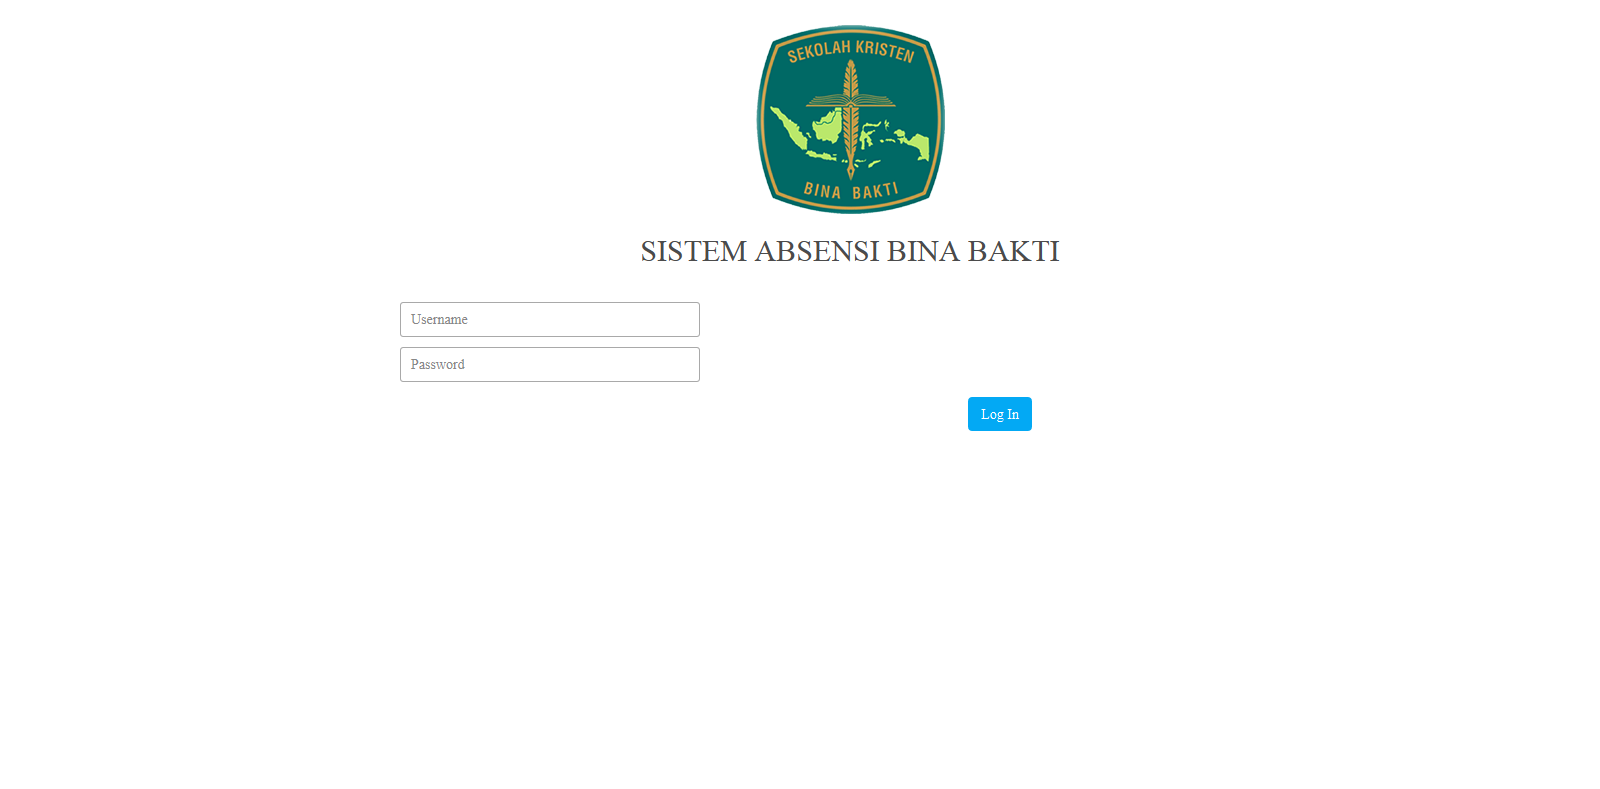
\includegraphics[width=1.00\textwidth]{gambar/1.png}}
	\caption{Halaman \textit{Log In}}
	\label{fig:page1}
\end{figure}	

Keterangan:
\begin{enumerate}
	\item \textit{Field} untuk diisi dengan \textit{username} dari akun pengguna yang telah terdaftar di Sistem Informasi Absensi Bina Bakti. Pengguna dapat didaftarkan oleh pengguna yang memiliki peran sebagai admin melalui halaman \textit{manage user} (subbab \ref{sec:page5}).
	\item \textit{Field} untuk diisi dengan \textit{password} yang sesuai.
	\item Tombol untuk \textit{log in}. Jika pengguna memasukkan \textit{username} dan \textit{password} yang tepat, maka pengguna akan diarahkan ke halaman \textit{dashboard} (Subbab \ref{sec:page2}).
\end{enumerate}

%--------------------------------------------------

\subsubsection{Halaman \textit{Dashboard}}
\label{sec:page2}

\begin{figure}[H]
	\centering
		\fbox{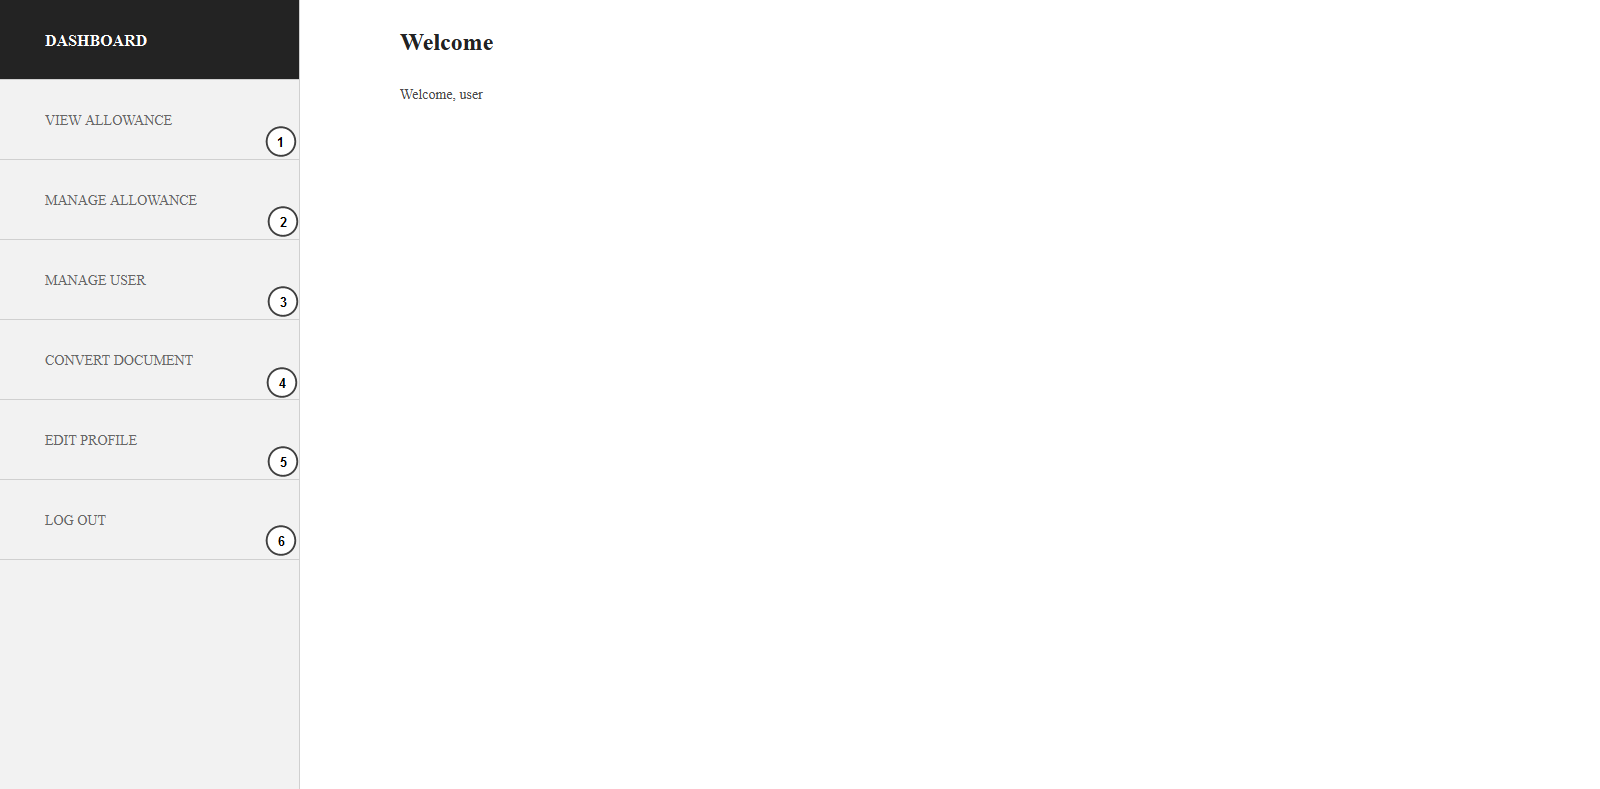
\includegraphics[width=1.00\textwidth]{gambar/2.png}}
	\caption{Halaman \textit{Dashboard}}
	\label{fig:page2}
\end{figure}	

Keterangan:
\begin{enumerate}
	\item \textit{Tab} untuk navigasi ke halaman \textit{view allowance} (Subbab \ref{sec:page3}).
	\item \textit{Tab} untuk navigasi ke halaman \textit{manage allowance} (Subbab \ref{sec:page4}).
	\item \textit{Tab} untuk navigasi ke halaman \textit{manage user} (Subbab \ref{sec:page5}).
	\item \textit{Tab} untuk navigasi ke halaman \textit{convert document} (Subbab \ref{sec:page6}).
	\item \textit{Tab} untuk navigasi ke halaman \textit{edit profile} (Subbab \ref{sec:page7}).
	\item \textit{Tab} untuk \textit{log out}.	Pengguna akan diarahkan ke halaman \textit{log in} (Subbab \ref{sec:page1}).
\end{enumerate}

%--------------------------------------------------

\subsubsection{Halaman \textit{View Allowance}}
\label{sec:page3}

\begin{figure}[H]
	\centering
		\fbox{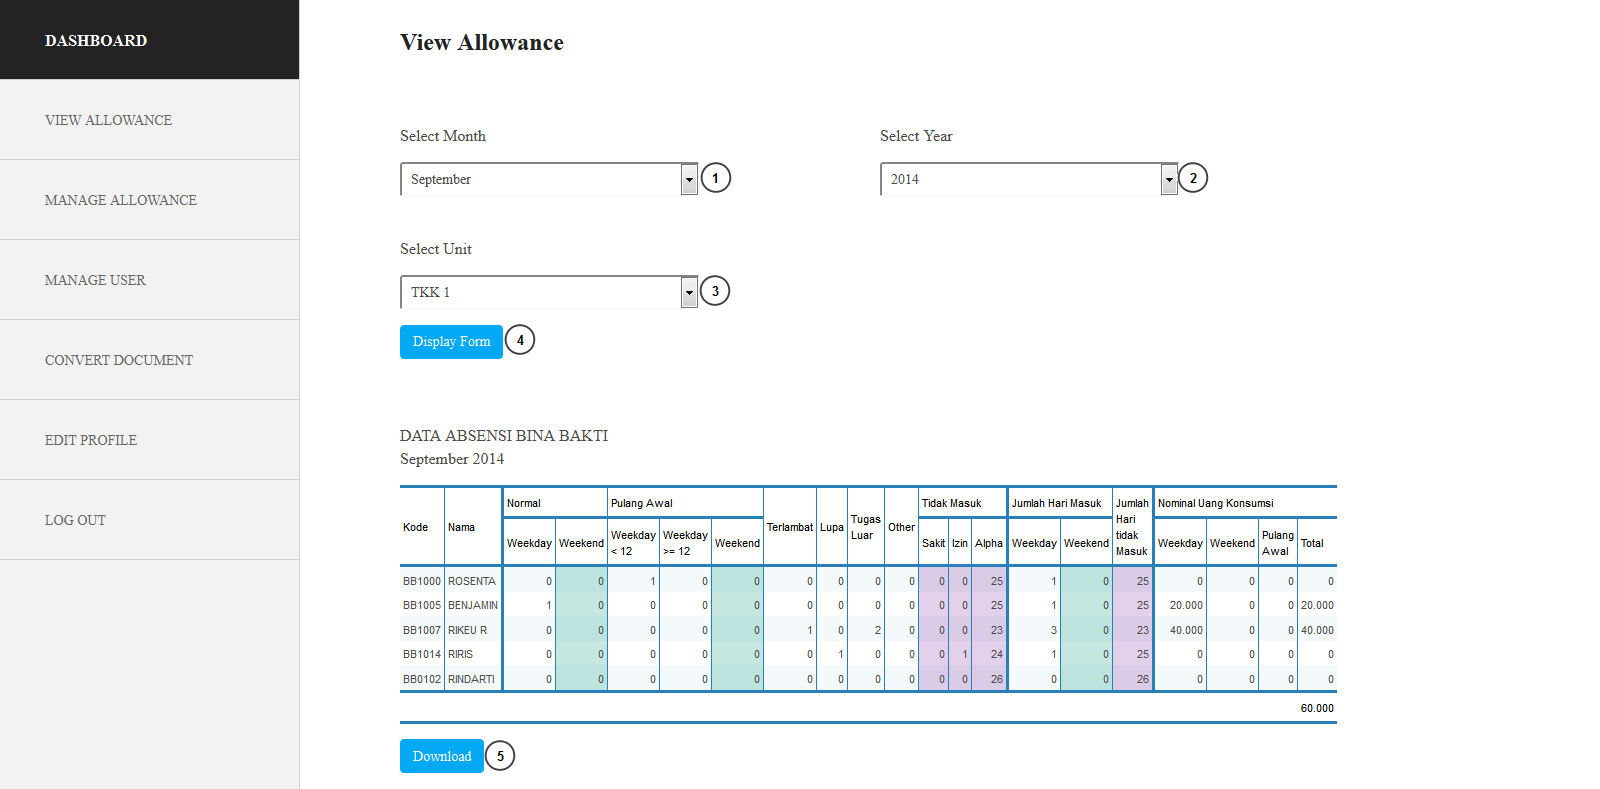
\includegraphics[width=1.00\textwidth]{gambar/3.png}}
	\caption{Halaman \textit{View Allowance}}
	\label{fig:page3}
\end{figure}	

Keterangan:
\begin{enumerate}
	\item \textit{Combo box} untuk menentukan bulan.
	\item \textit{Combo box} untuk menentukan tahun.
	\item \textit{Combo box} untuk menentukan unit.
	\item Tombol untuk menampilkan tabel Data Absensi Bina Bakti sesuai dengan bulan, tahun, dan unit yang dipilih pengguna.
	\item Tombol untuk mengunduh tabel Data Absensi Bina Bakti sesuai dengan bulan, tahun, dan unit yang dipilih pengguna. Tabel tersebut dapat diunduh sebagai \textit{file} dengan format ``.csv'' yang dapat digunakan oleh Microsoft Excel. 
\end{enumerate}

%--------------------------------------------------

\subsubsection{Halaman \textit{Manage Allowance}}
\label{sec:page4}

\begin{figure}[H]
	\centering
		\fbox{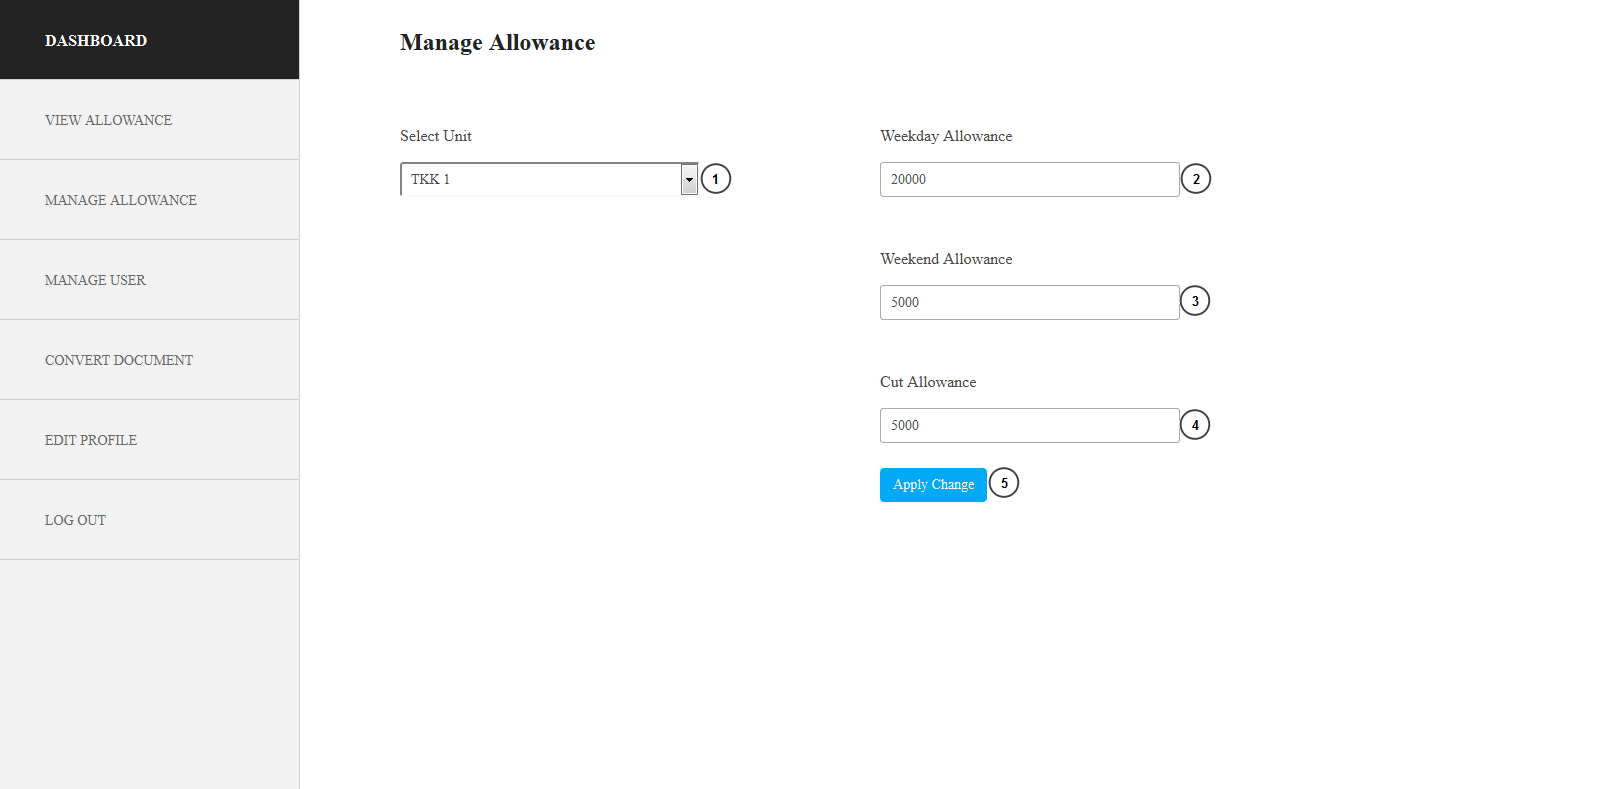
\includegraphics[width=1.00\textwidth]{gambar/4.png}}
	\caption{Halaman \textit{Manage Allowance}}
	\label{fig:page4}
\end{figure}	

Keterangan:
\begin{enumerate}
	\item \textit{Combo box} untuk menentukan kategori jam kerja.
	\item \textit{Field} untuk menampilkan nominal uang konsumsi hari kerja (khusus untuk unit yang dipilih pengguna). Pengguna dapat mengubah besaran nominalnya.
	\item \textit{Field} untuk menampilkan nominal uang konsumsi akhir pekan (khusus untuk unit yang dipilih pengguna). Pengguna dapat mengubah besaran nominalnya.
	\item \textit{Field} untuk menampilkan nominal uang konsumsi yang dipotong jika karyawan pulang awal di atas jam 12 (khusus untuk unit yang dipilih pengguna). Pengguna dapat mengubah besaran nominalnya.
	\item Tombol untuk menyimpan perubahan nominal uang konsumsi.
\end{enumerate}

%--------------------------------------------------

\subsubsection{Halaman \textit{Manage User}}
\label{sec:page5}

\begin{figure}[H]
	\centering
		\fbox{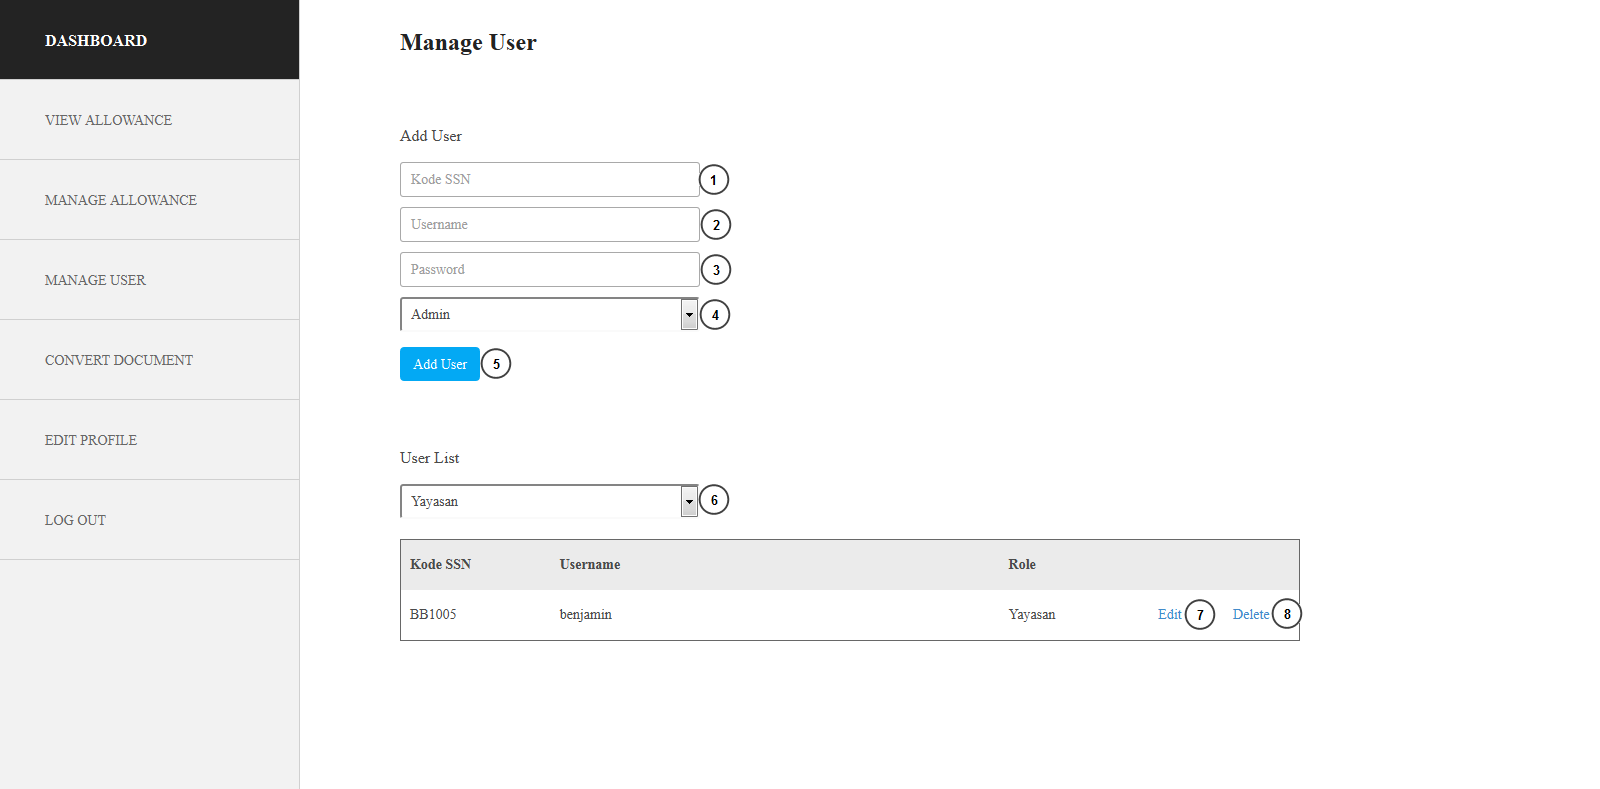
\includegraphics[width=1.00\textwidth]{gambar/5a.png}}
	\caption{Halaman \textit{Manage User}}
	\label{fig:page5a}
\end{figure}	

Keterangan:
\begin{enumerate}
	\item \textit{Field} untuk diisi dengan kode SSN karyawan dari akun pengguna yang akan ditambahkan.
	\item \textit{Field} untuk diisi dengan \textit{username} dari akun pengguna yang akan ditambahkan. \textit{Username} ini bersifat unik dan harus berbeda untuk setiap karyawan.
	\item \textit{Field} untuk diisi dengan \textit{password} dari akun pengguna yang akan ditambahkan.
	\item \textit{Combo box} untuk menentukan peran dari akun pengguna yang akan ditambahkan.
	\item Tombol untuk menambah data akun pengguna baru ke basis data.
	\item \textit{Combo box} untuk menentukan peran dan menampilkan daftar akun pengguna yang memiliki peran tersebut di basis data.	
	\item Tombol untuk mengubah data akun pengguna. Tombol ini akan memunculkan \textit{pop up} yang dapat digunakan untuk mengubah data akun pengguna (Gambar \ref{fig:page5b}).
	\item Tombol untuk menghapus data akun pengguna.
\end{enumerate}

\begin{figure}[H]
	\centering
		\fbox{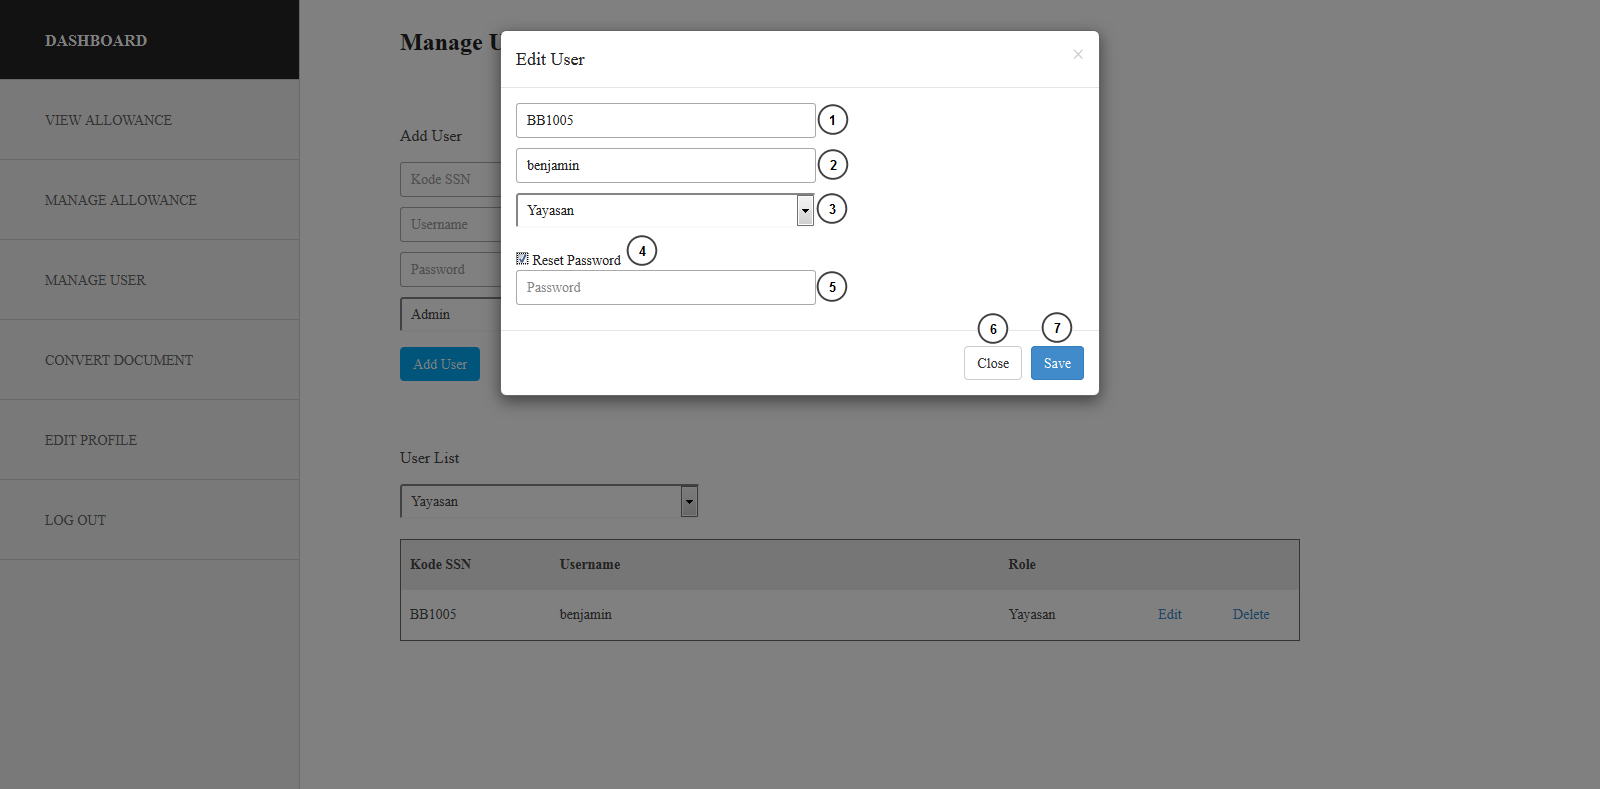
\includegraphics[width=1.00\textwidth]{gambar/5b.png}}
	\caption{Halaman \textit{Manage User} (\textit{Pop Up})}
	\label{fig:page5b}
\end{figure}	

Keterangan:
\begin{enumerate}
	\item \textit{Field} untuk menampilkan kode SSN karyawan dari akun pengguna yang sedang diedit. Pengguna dapat mengubahnya.
	\item \textit{Field} untuk menampilkan \textit{username} dari akun pengguna yang sedang diedit. Pengguna dapat mengubahnya.
	\item \textit{Combo box} untuk menampilkan \textit{role} dari akun pengguna yang sedang diedit. Pengguna dapat mengubahnya.
	\item \textit{Checkbox} untuk menentukan apakah perlu pengubahan \textit{password}. Jika \textit{checkbox} ini ditandai, maka \textit{field} untuk diisi dengan \textit{password} baru akan ditampilkan, jika sebaliknya maka \textit{field} tersebut akan disembunyikan.
	\item \textit{Field} untuk diisi dengan \textit{password} baru.
	\item Tombol untuk membatalkan perubahan yang dilakukan dan menutup \textit{pop up} ini. 
	\item Tombol untuk menyimpan perubahan yang dilakukan ke basis data dan menutup \textit{pop up} ini. 
\end{enumerate}

%--------------------------------------------------

\subsubsection{Halaman \textit{Convert Document}}
\label{sec:page6}

\begin{figure}[H]
	\centering
		\fbox{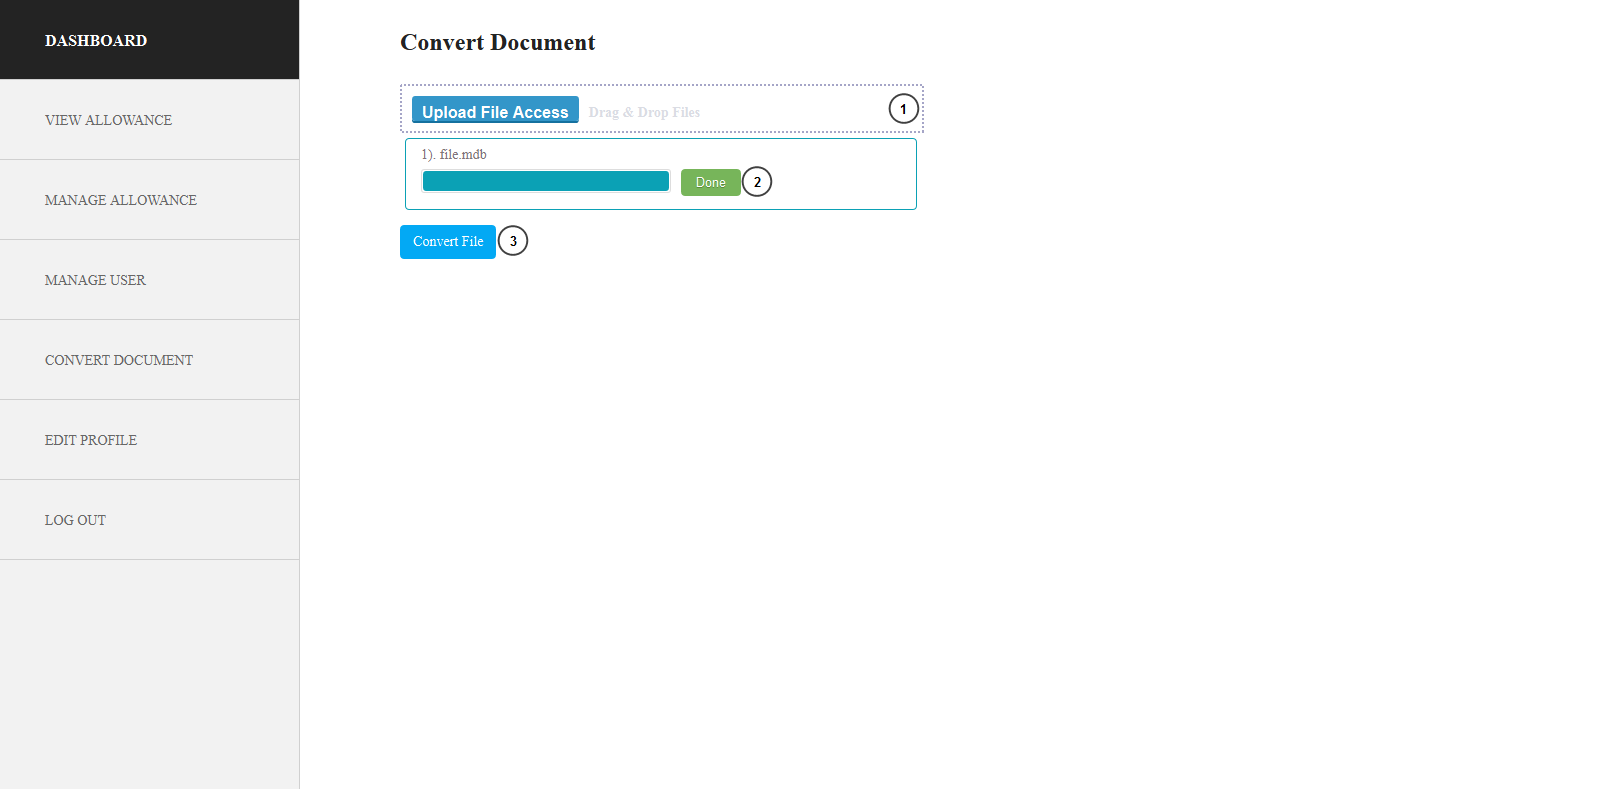
\includegraphics[width=1.00\textwidth]{gambar/6.png}}
	\caption{Halaman \textit{Convert Document}}
	\label{fig:page6}
\end{figure}	

Keterangan:
\begin{enumerate}
	\item Tombol untuk memilih \textit{file} basis data (berekstensi ``.mdb''). Pengguna dapat menekan tombol ini ataupun melakukan \textit{drag} dan \textit{drop file} ke area tombol ini.
	\item Tombol disertai \textit{progress bar} untuk memastikan bahwa \textit{file} telah selesai diunggah. 
	\item Tombol untuk memulai konversi data yang disimpan di \textit{file} tersebut menjadi data di MySql.
\end{enumerate}

%--------------------------------------------------

\subsubsection{Halaman \textit{Edit Profile}}
\label{sec:page7}

\begin{figure}[H]
	\centering
		\fbox{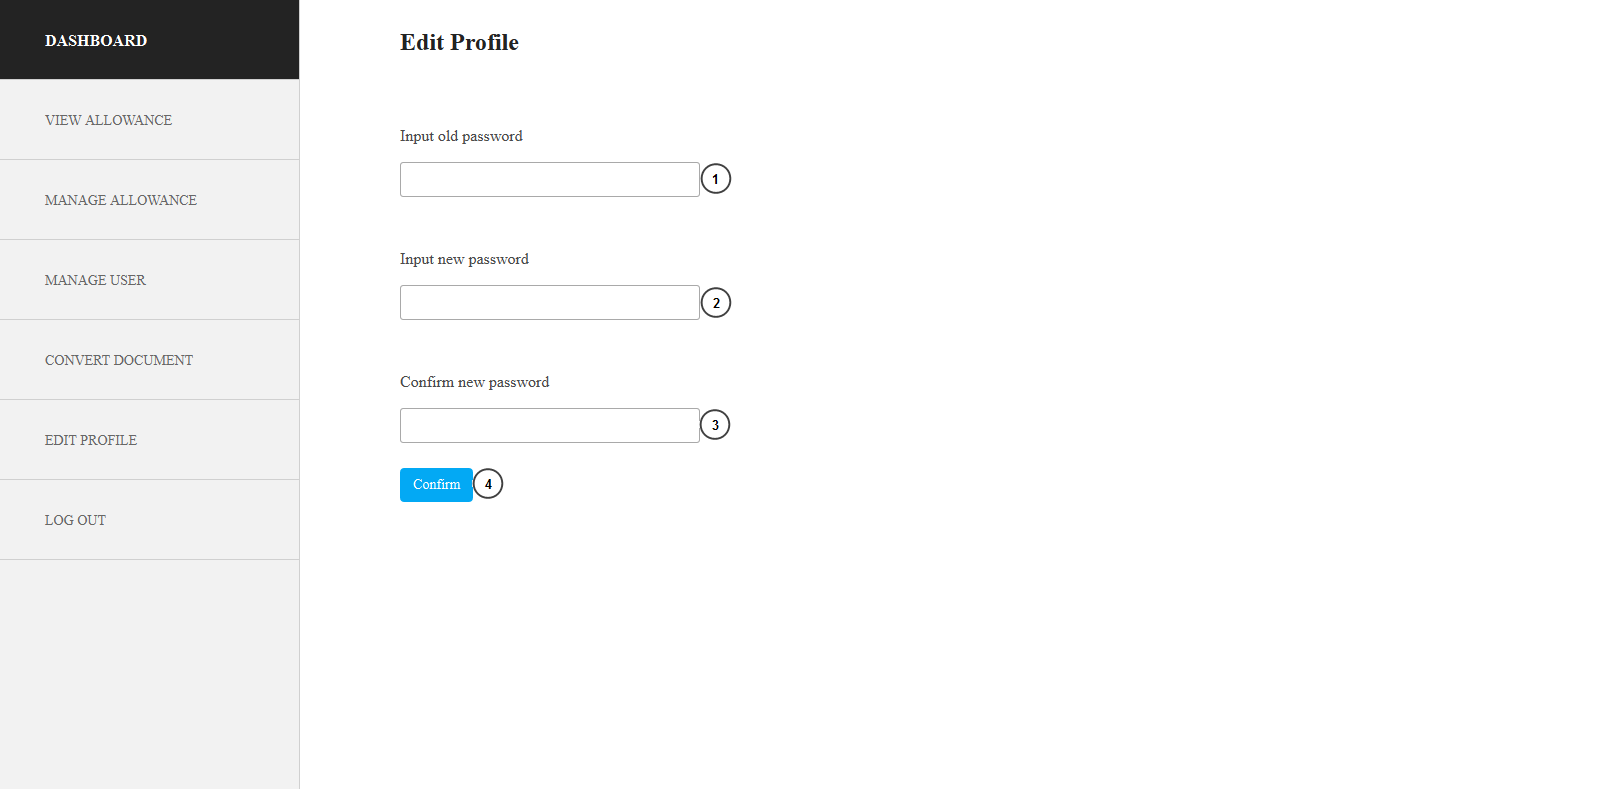
\includegraphics[width=1.00\textwidth]{gambar/7.png}}
	\caption{Halaman \textit{Edit Profile}}
	\label{fig:page7}
\end{figure}	

Keterangan:
\begin{enumerate}
	\item \textit{Field} untuk diisi dengan \textit{password} lama.
	\item \textit{Field} untuk diisi dengan \textit{password} baru.
	\item \textit{Field} untuk diisi dengan \textit{password} baru.	
	\item Tombol untuk menyimpan \textit{password} baru pengguna ke basis data.
\end{enumerate}
